\documentclass[12pt,letterpaper,english]{article}
\usepackage[T1]{fontenc}
\usepackage[latin9]{inputenc}
\pagestyle{empty}
\usepackage{amsmath}
\usepackage{amssymb}
\usepackage{graphicx}
\usepackage{bm}
\usepackage{multicol}
\usepackage{enumitem}

\usepackage{hyperref}
\hypersetup{
    colorlinks=true,
    linkcolor=blue,
    filecolor=magenta,      
    urlcolor=cyan,
}


\newcommand{\norm}[1]{\lVert#1\rVert}

\makeatletter

\special{papersize=\the\paperwidth,\the\paperheight}



\textwidth6.5in\textheight9in\topmargin-.25in\oddsidemargin0in\evensidemargin0in\parskip5pt\parindent0pt


\usepackage{fancyhdr}
\pagestyle{fancy}
\lhead{Reconfigurable Mechanical Vibrations Laboratory Kit}
\rhead{}


\usepackage{lastpage}
 
  
\rfoot{Page \thepage \hspace{1pt} of \pageref{LastPage}}

%\rfoot{\small }
\lfoot{Mechanical Vibrations: Lab 3}
\cfoot{}




\usepackage{babel}


\makeatother

\usepackage{babel}
\begin{document}
\global\long\def\Re{{\rm {Re }}}
 \global\long\def\cL{{\cal L}}
 \global\long\def\sq{{\rm {sq}}}
 \global\long\def\bfx{{\bf x}}
 \global\long\def\bfi{{\bf i}}
 \global\long\def\bfj{{\bf j}}


\begin{center}
\textbf{\large Lab Assignment 3:  Nonlinear Oscillator}
\par\end{center}{\large \par}


The goal of this demo will be to investigate the dynamics of a nonlinear oscillator.  This system, as depicted below, can be modeled by a Duffing equation where there is a nonlinear spring term in the governing equation.

\begin{center}
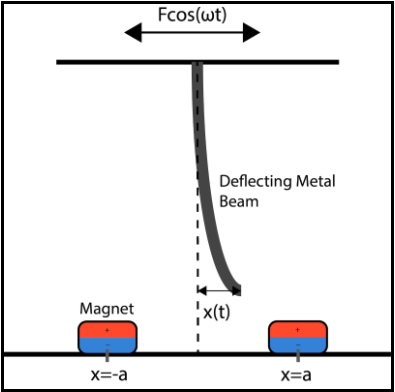
\includegraphics[width=3in]{schematic.png}
\end{center}

First, read through section E3 (``Nonlinear Oscillator Demo'') in the Assembly Guide to learn how to modify the existing housing to incorporate the necessary components for this demo. The fully assembled rig should look like this:

\begin{center}
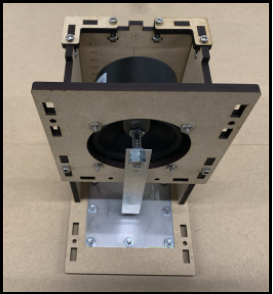
\includegraphics[width=3in]{lab3a.png}
\end{center}

Note that as detailed in the assembly guide, you will need to add one or two layers of nuts at the bottom of the two magnets such that the height from the top of the beam to the top surface of the magnets is around 7mm to 7.5mm. (For reference, see the diagram below which includes a way to estimate 7mm using the components of your kit.)  Note that the mounting hole on the sheet metal beam has a diameter larger than 1/4'', which also allows additional freedom for fine tuning this spacing. Furthermore, elevating the magnets will make it easier to move the magnets on the steel plate. When placing the magnets, it may be helpful to rotate the beam to an angle so that the magnets do not interact with it. Feel free to add as many nuts as you feel are helpful for stability (see images below). 

\begin{center}
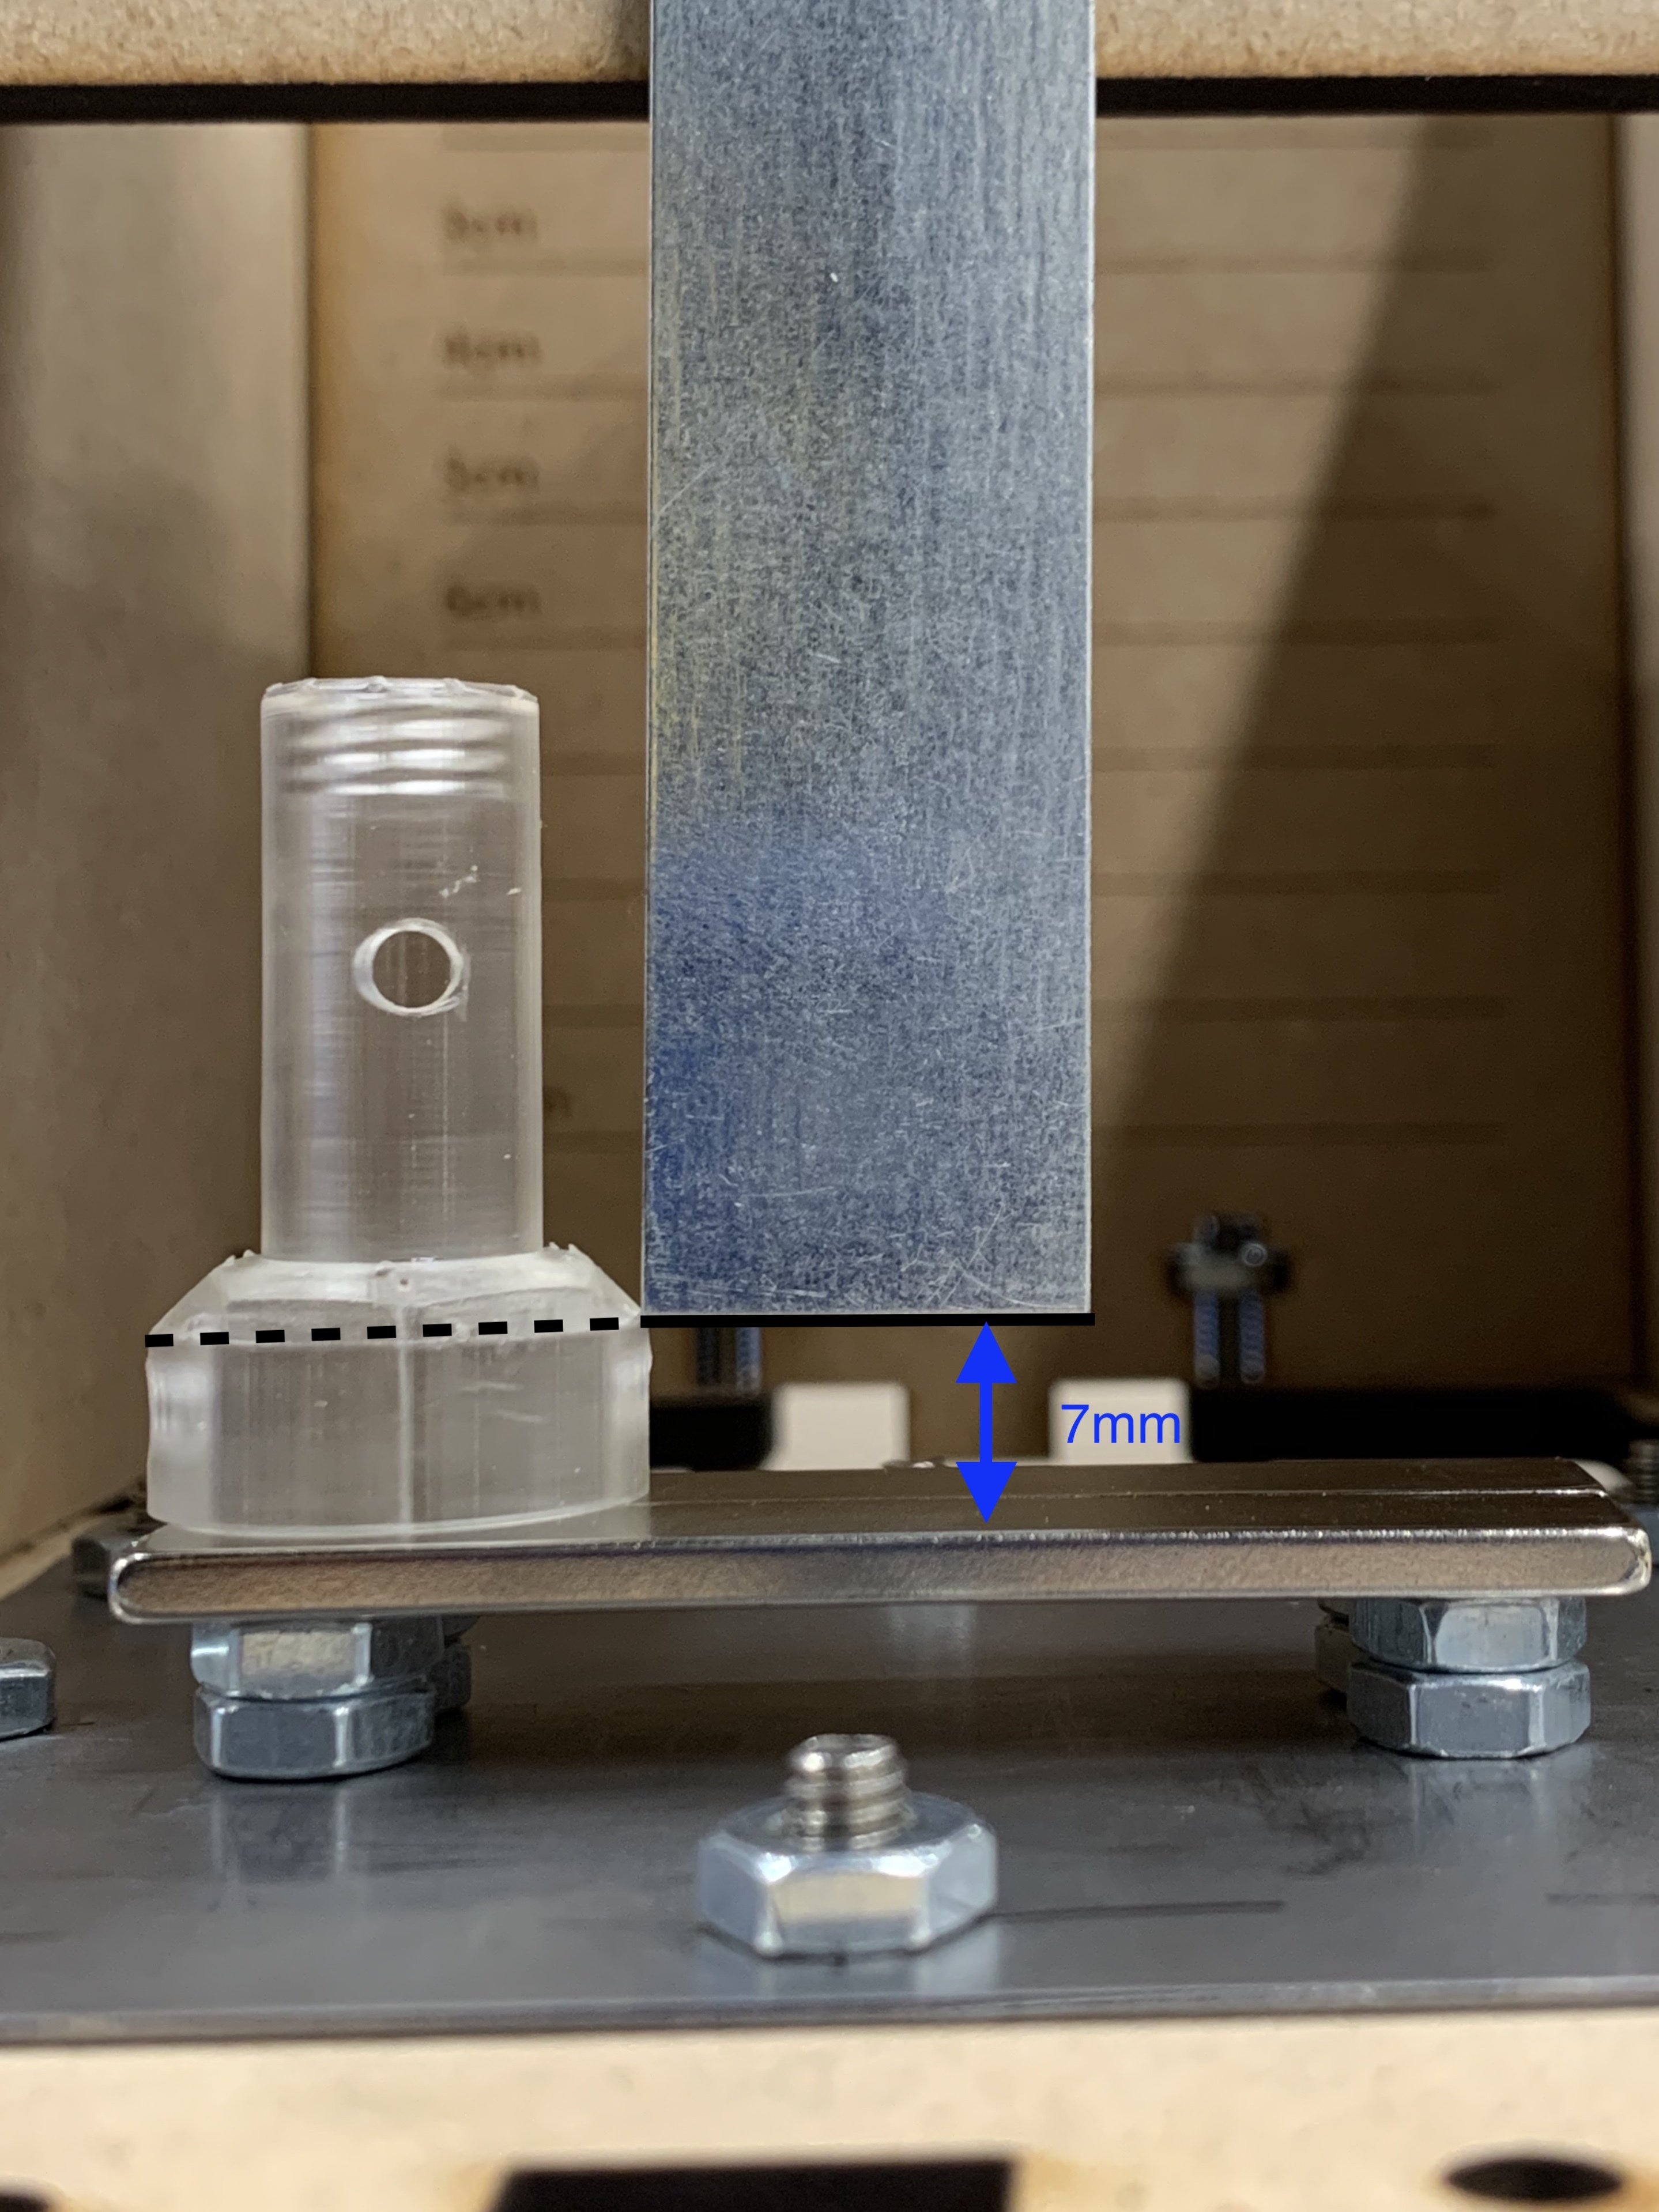
\includegraphics[width=1.75in]{lab3c.jpg}
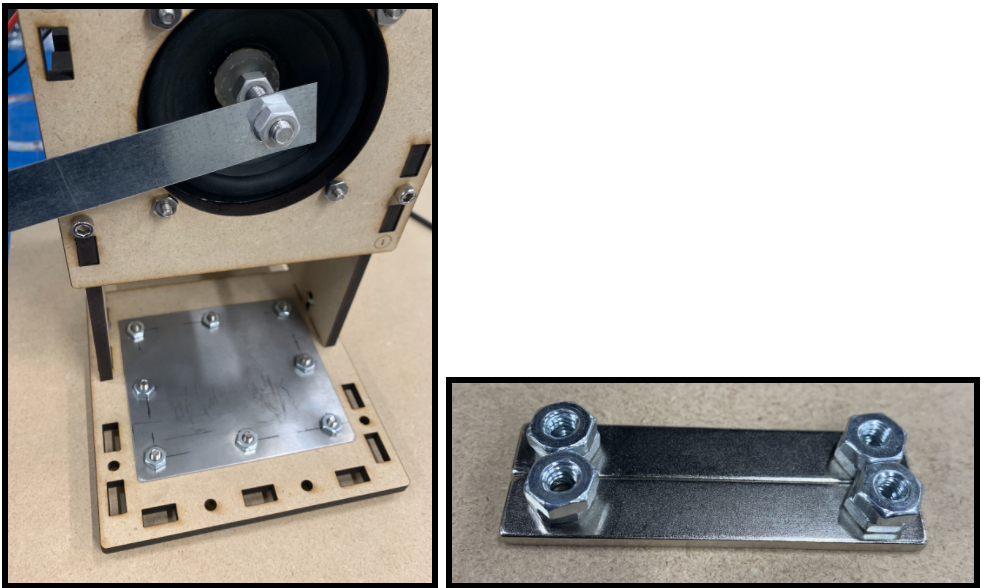
\includegraphics[width=3.5in]{lab3b.png}
\end{center}

Next, carefully place the magnets on the steel plate directly below the sheet metal beam. The response of the beam is highly sensitive to the height and location of these magnets. To first ensure that the height of the magnet is suitable (if it is around 7mm to 7.5mm it should be fine), by hand, flick the beam from one equilibrium position to the other as depicted below. You should be able to ``feel'' the potential well corresponding to each equilibrium position. If you are finding that the beam tends to move away from one equilibrium position, adjust the location of the magnets slightly biasing it towards that particular side. 

{\small *Note that we will fine tune the magnets position later on and that this is just to get a sense of the two stable equilibrium positions.  Also note that the speaker membrane will deflect as you move the beam.}

\begin{center}
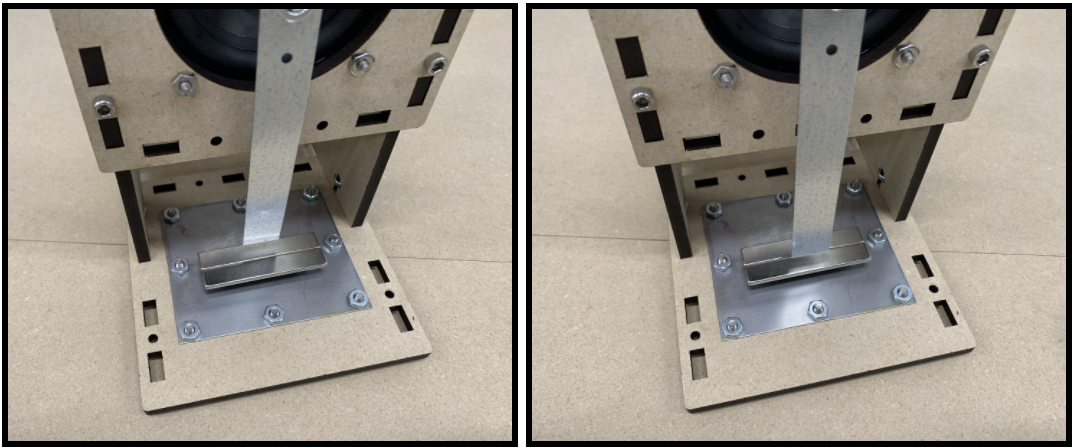
\includegraphics[width=5.5in]{lab3d.png}
\end{center}



The motion of the beam can be modeled as a one degree of freedom linear harmonic oscillator where our coordinate of interest is the tip position $x(t)$.  Assume the beam has an effective spring constant $k_s$, structural damping coefficient $c$, and effective mass $m$.

The additional lateral force that the tip of the beam feels due to the presence of the two magnets can be modeled approximately by the following nonlinear force law
\begin{equation}
F_m(x)=k_m \left[1-\left(\frac{x}{d}\right)^2\right]x \nonumber
\end{equation}
where $k_m\geq0$ is a parameter that depends on the relative height between the magnets and the beam.  For instance, as the magnets are moved further away from the beam $k_m \rightarrow 0$.


\begin{enumerate}
\item Write the down the governing ODE for the system, including the magnetic force term $F_m$.  Determine the position of all equilibrium points and their stability as a function of the magnetic parameter $k_m$.  Describe what happens physically as $k_m$ is gradually increased starting from 0 (corresponding physically to bringing the magnets closer and closer to the beam).
\end{enumerate}

The equation of motion for this problem has the form of Duffing's equation, which is a forced nonlinear oscillator that includes a cubic ($x^3$) nonlinearity.  The general form of the Duffing equation takes the following mathematical form:
\begin{equation}
\ddot{x}+\delta \dot{x} +\alpha x + \beta x^3 = \gamma \cos \omega t \nonumber.
\end{equation}
\begin{enumerate}[resume]
\item Driving the experiment at 20 Hz, slowly increase the driving amplitude (using slightly detuned strobing).  You should see three regimes as the amplitude is increased progressively: (1) small oscillations about one of the equilibrium positions, (2) chaotic/irregular oscillation between the two equilibrium positions, (3) large \emph{periodic} oscillations passing over both equilibrium positions on each cycle.  If you do not see these three regimes clearly, you may need to adjust the position of your magnets or the gap between the beam and magnets slightly.  Repeat the sweep with the magnets removed to isolate the influence of the magnets (i.e. nonlinearity).

\vspace{0.05in}

Simulate Duffing's equation using values $\delta=0.5$, $\alpha=-1$, $\beta = 0.2$, and $\omega=1$.  By increasing $\gamma$ generate three phase portraits that correspond qualitatively to the 3 regimes you observe in the experiment.  Note that in the simulation there is always an initial \emph{transient} period before it locks into a specific mode so make sure to run the simulation long enough to discern the steady-state behavior.  Include images of the three phase plots (labeled with value of $\gamma$ used) with your assignment.

\item Now with full freedom on driving frequency and tip spacing, identify another possible \emph{qualitative} behavior in the experiment.  You can use the strobing (synchronized and/or detuned) to help identify the behavior as best as possible.  Then similarly with full freedom on the numerical parameters, recover the qualitative mode you observe by simulating Duffing's equation.  Take a video (slo-mo if you have it on your phone) of the new mode and image of the corresponding phase portrait from your simulation to include with your assignment.

\item Provide feedback or ideas (positive and/or areas for improvement) on the setup process and nonlinear oscillation lab. 

\end{enumerate}


\vspace{0.5 in}


{\it \small Application note: A very similar type of ``bi-stable system'' has been proposed as a method for harvesting energy from mechanical vibration as shown below. The nonlinearity of the system can be exploited to harvest energy effectively over a broader range of frequency input as compared to a linear oscillator which is only effective near its natural frequency.  This type of small-scale energy harvester is expected to find applications for powering sensors where another power source cannot be used, such as in implantable devices.}

\begin{center}
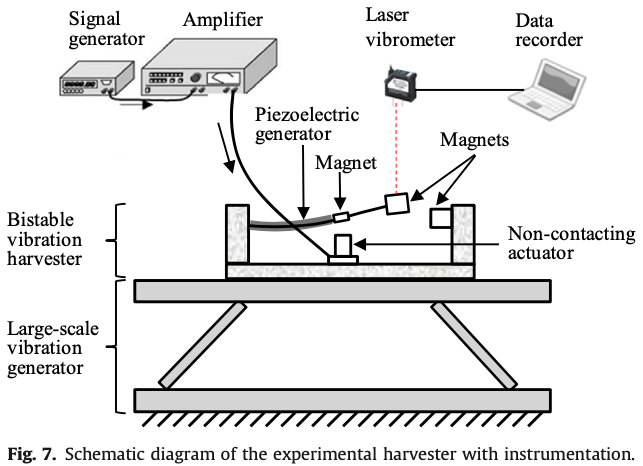
\includegraphics[width=2.75in]{harvest.png}
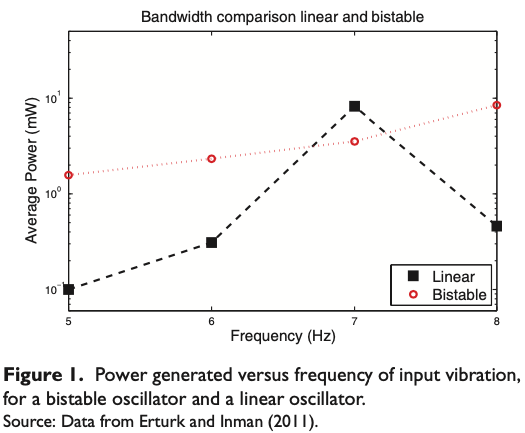
\includegraphics[width=2.5in]{data.png}
\end{center}

{\it \scriptsize	 Figure credit: (left) Zheng, R., Nakano, K., Hu, H., Su, D. and Cartmell, M.P., 2014. An application of stochastic resonance for energy harvesting in a bistable vibrating system. Journal of Sound and Vibration, 333(12), pp.2568-2587.  (right) Pellegrini, S.P., Tolou, N., Schenk, M. and Herder, J.L., 2013. Bistable vibration energy harvesters: a review. Journal of Intelligent Material Systems and Structures, 24(11), pp.1303-1312. }







\end{document}
